% ================
% Landon Buell
% 
% 
% 26 May 2020
% ================

\documentclass[12pt,letterpaper]{article}

\usepackage{amsmath,amssymb,amsfonts}
\usepackage{algorithmic}
\usepackage{graphicx}
\usepackage{textcomp}
\usepackage{xcolor}
\usepackage{subfigure}
\usepackage{pgf}
\usepackage{multirow}

\usepackage[left=2.5cm,right=2.5cm,top=2.5cm]{geometry}

\begin{document}


\textcolor{red}{Place for Landon}

% BEGIN LANDON'S ADDITIONS (28-MAY-2020-21:55) 

\subsection{Case Study 1: Multilayer Perceptron}

The purpose of this case study was to develop an understanding for how the multilayer perceptron (MLP) neural network architecture is affected by a \textit{bit muting} attack function that seeks to manipulate the values of a floating-point number at a binary level. In the case of this experiment, we have chosen to model a function that forces the most-significant-bit (MSB) in the exponent of floating-point number to be muted to $0$. In each MLP model, numerical values were stored as double precision floating-point numbers as per the IEEE 754 standard. 
%Note that the exponent value was set to $0$, rather than subtract $1023$ to save further computation time and avoid invalid ranges when converting the mantissa and exponent back into it's floating-point counterpart.
When mute MSB attack occurs on a single floating-point number, it is then constrained to lie on the open interval $(-1,+1)$. A map of input values against MSB output values is shown in Fig.~\ref{fig-MUTEMSB}. The inputs are a subset of the possible values of a double precision floating-point numbers for visual ease.

\begin{figure}[h]
	\centering
	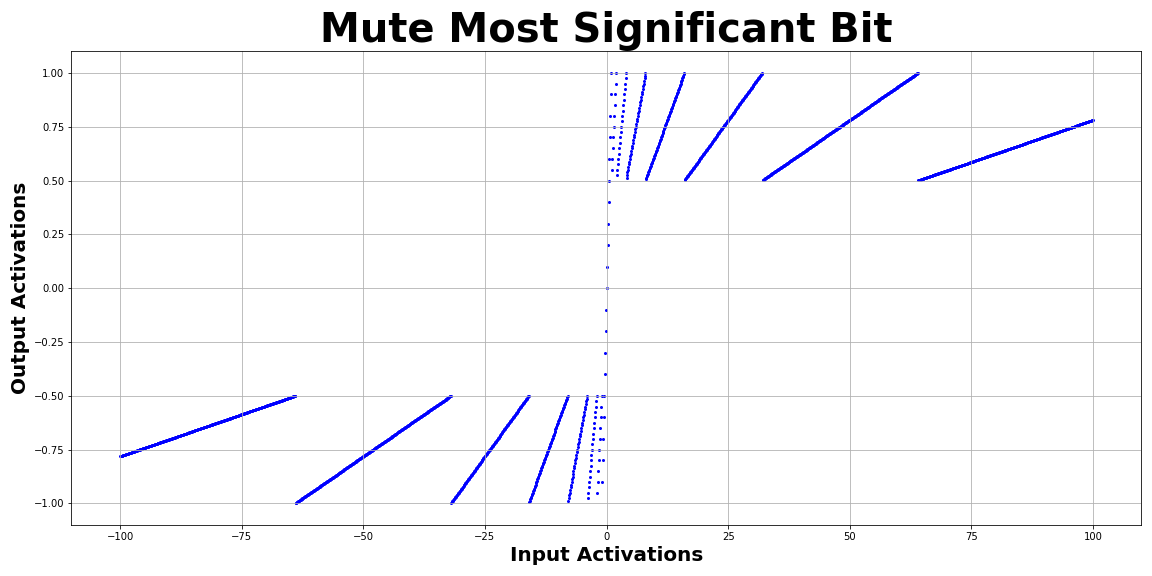
\includegraphics[width=0.9\columnwidth]{Fig/Mute_Most_Significant_Bit.png}
	%\textcolor{red}{Please Help me with the formatting of this image!}
	\label{fig-MUTEMSB}
	\caption{Input versus output values of double precision floating-point numbers subject to the \textit{mute most-significant-bit} attack function. Inputs shown are $-1000$ to $+1000$.}
\end{figure}

\subsubsection{Experimental Setup}
The MLP neural network model is composed of multiple layers of \textit{neurons}, that each contain a real-valued floating-point number called an \textit{activation}.  
In general, given a layer of activations $\vec{x}^{(l)}$ (The superscript is used as a layer index), the activations in the next sequential layer, $\vec{x}^{(l+1)}$, are produced with weighting matrix $\hat{W}^{(l)}$, bias vector $\vec{b}^{(l)}$, and activation function $f$ such that:

\begin{equation}
\label{eq-feed-forward}
\vec{x}^{(l+1)} = f \Big( \hat{W}^{(l)} \vec{x}^{(l)} + \vec{b}^{(l)} \Big)
\end{equation}

The recurrence of Eq.(\ref{eq-feed-forward}) is used to pass information forward through the network. In a network with $L$ layers, raw information is given with $\vec{x}^{(0)}$ and the network's prediction is given by the final layer, $\vec{x}^{(L-1)}$.

The Multilayer Perceptron network must then find a series of parameters, which are the elements in all weighting matrices and all bias vectors, that allows for a given sample to produce a low value for a given \textit{Loss function}. The loss function measures the difference between a networks given output and expected output; with better trained networks producing generally low loss values over a set of samples. The process of finding the values is called \textit{optimization}. There are many different algorithms that perform optimization, and for this experiment, we have chosen to use \textit{Stochastic Gradient Descent} (SGD) due to its widespread use and versatility. This method uses successive passes over a training data set to iterativly update model parameters such that they allow for a convergence is the lowest possible loss value.

To model a bit-muting attack, we introduce and \textit{attack function} that acts in the matrix-vector product 
in Eq.(\ref{eq-feed-forward}). When a Boolean \textit{trigger condition} parameter is met, the MSB attack as described above, Eq.(\ref{eq-feed-forward}) is instead replaced with it's attack variant:

\begin{equation}
\label{eq-Attack}
\vec{x}^{(l+1)} = f \Big( A \big[ \hat{W}^{(l)} \vec{x}^{(l)} \big] + \vec{b}^{(l)} \Big)
\end{equation}

Where $A$ is the attack function, applied element-wise to each object in it's argument. 

For a practical demonstration of this attack function, we have tested it on variants of an image classification neural network. Each network was given of subset of training images from the MNIST data set, each containing a pixelized handwritten digit, labeled $0$ through $9$ according to the digit in that image. Each model was then trained on $6400$ similar, but non-identical images for evaluation. A subset of samples is visualized with a binary color map in Fig.~\ref{MNIST}. 

\begin{figure}[h]
	\label{MNIST}
	\centering
	%\textcolor{red}{Please Help me with the formatting of this image!}
	%\includegraphics[scale=0.3]{MNIST}
	\includegraphics[width=0.9\columnwidth]{Fig/MNIST.png}
	\caption{Four MNIST figures shaped as $28$ pixel by $28$ pixel images, colored with a binary color map along with their corresponding labels.}
\end{figure}

Each sample is $28 \times 28$ pixels, each containing by a single integer $0$ through $255$ (which are transformed into floats when passed through the network). Images were shaped shaped into a $784 \times 1$ array object and used as input into the network. This means for each network model, there are always $784$ input neurons and $10$ output neurons (one for each class). To test different model architecture complexities, we tested networks containing $1$, $2$, $3$, and $4$ hidden layers (referred to as \textit{network depth}) and used $20$, $40$, $60$, $80$, $100$, and $120$ neurons per layer (referred to as \textit{neuron density} or \textit{network width}). Permutations of these parameters allowed for us to record behavior over $24$ unique MLP model variants.

\subsubsection{Impact of Bit-Muting Attack Classification Metrics}

\paragraph*{}To measure the impact of this type of attack on the image classifier model, we test a baseline classifier against a classifier subject to a random 50/50 trigger condition. From each variant, we have recorded the following metrics:

\begin{enumerate}
\item \textbf{Accumulated loss function for the final iteration.} This value measures the difference between expected outcome of the network and the given outcome. (Bounded to $[0,+\infty)$, lower is favorable)
\item \textbf{Average precision score all 10 classes.} Precision score is the ratio of true positive selections to total sections. It measures how many selected items are relevant to the given task. (Bounded $[0,1]$, higher is favorable)
\item \textbf{Average recall score for all 10 classes.} Recall score is the ratio of true positive selections to relevant sections. It measures how many relevant items in the given task are selected. (Bounded $[0,1]$, higher is favorable)
\end{enumerate} 

\paragraph*{}In each of the 12 model variants (2 layer depths, 6 densities), 50 models were trained, with the average, minimum and maximum values for each of the four metrics noted. The average for each metric, across each model depth and neuron density is plotted in fig. (\ref{results}). Note that the lack of a data point means that the value of that metric diverged to infinity or some other undefined value.

\begin{figure}[h]
	\centering
	%\textcolor{red}{Please Help me with the formatting of this image!}
	\subfigure[]{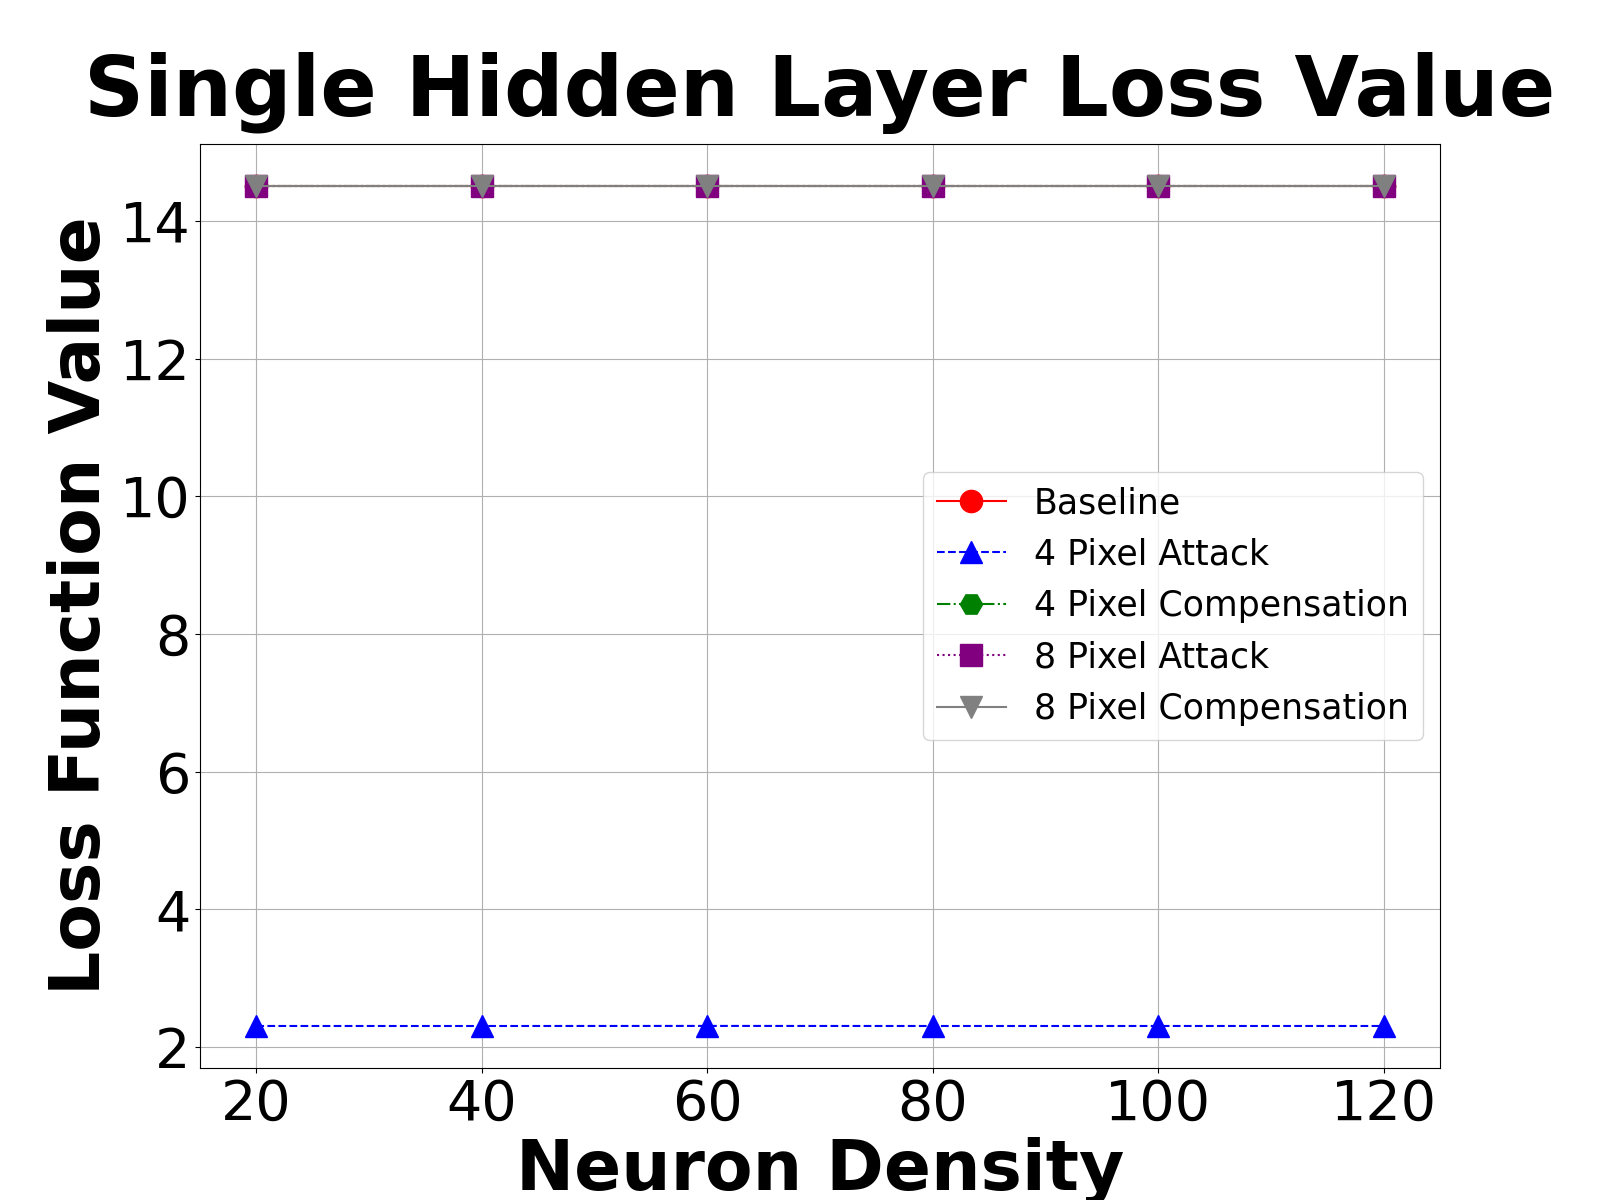
\includegraphics[width=0.45\columnwidth]{Fig/Single_Hidden_Layer_Loss_Value}}
	\subfigure[]{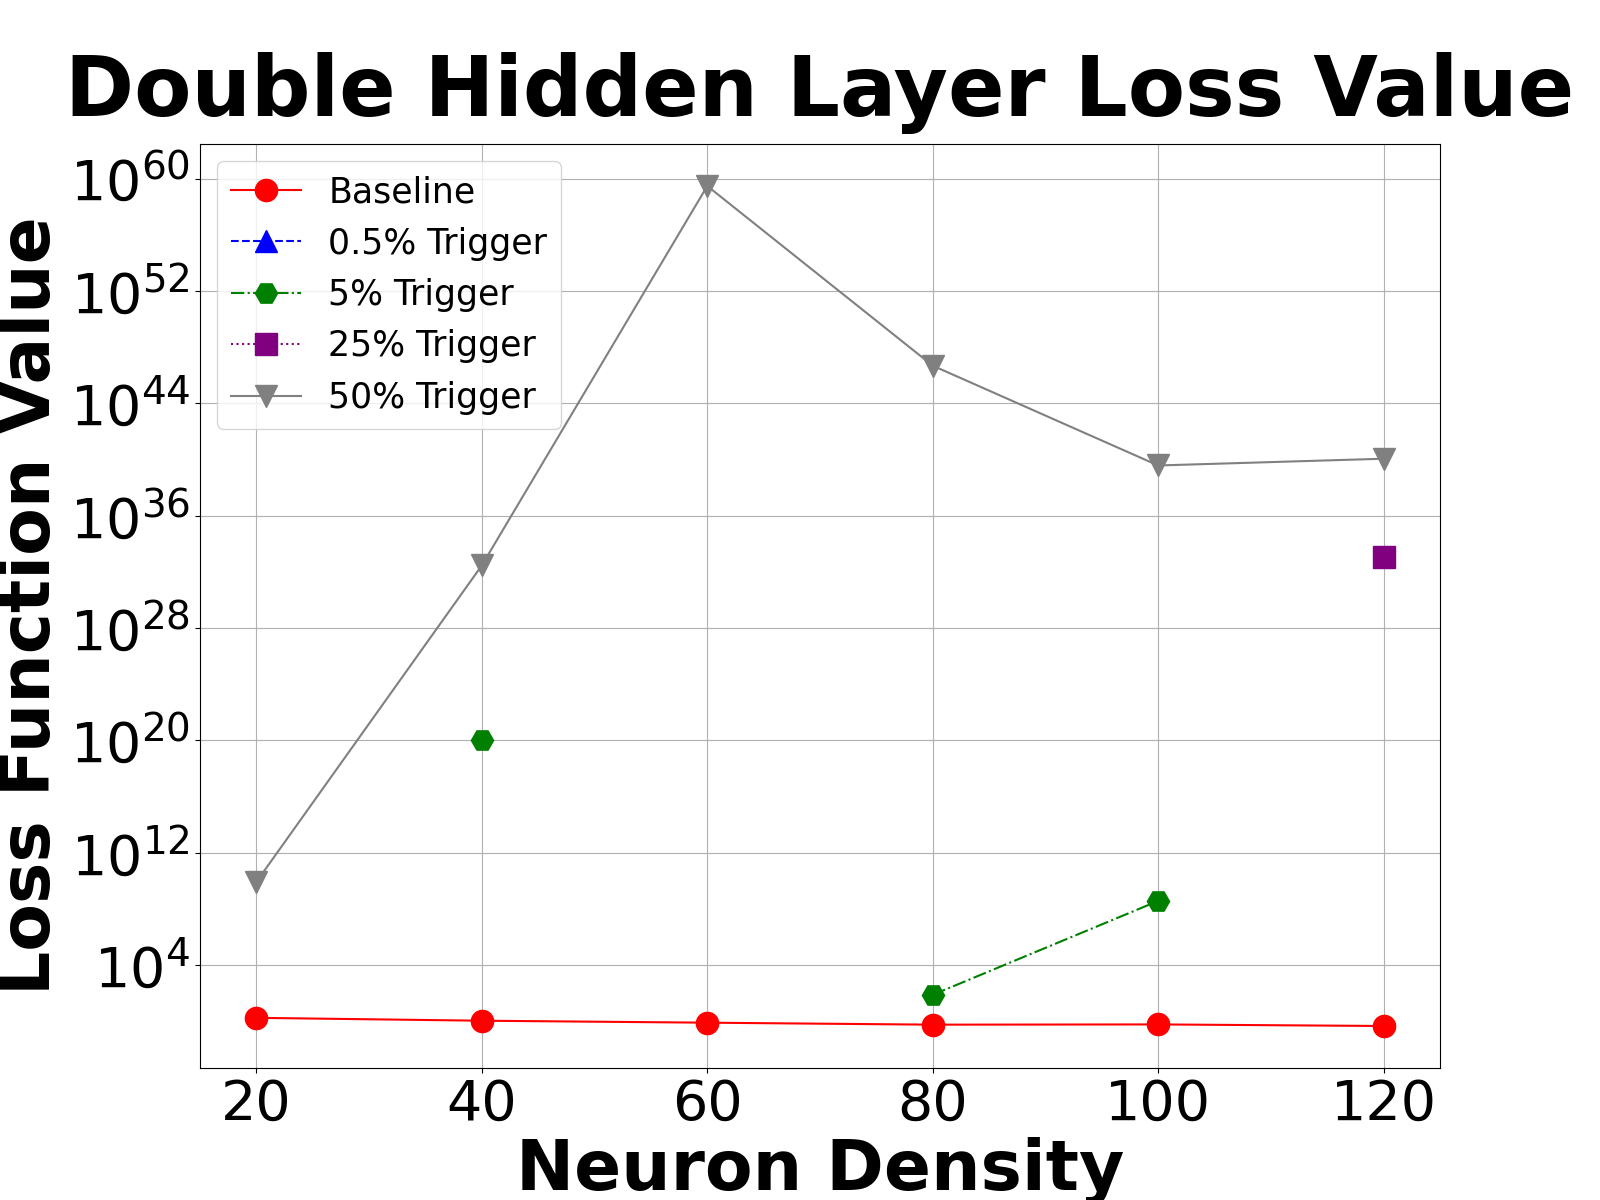
\includegraphics[width=0.45\columnwidth]{Fig/Double_Hidden_Layer_Loss_Value}}
	\subfigure[]{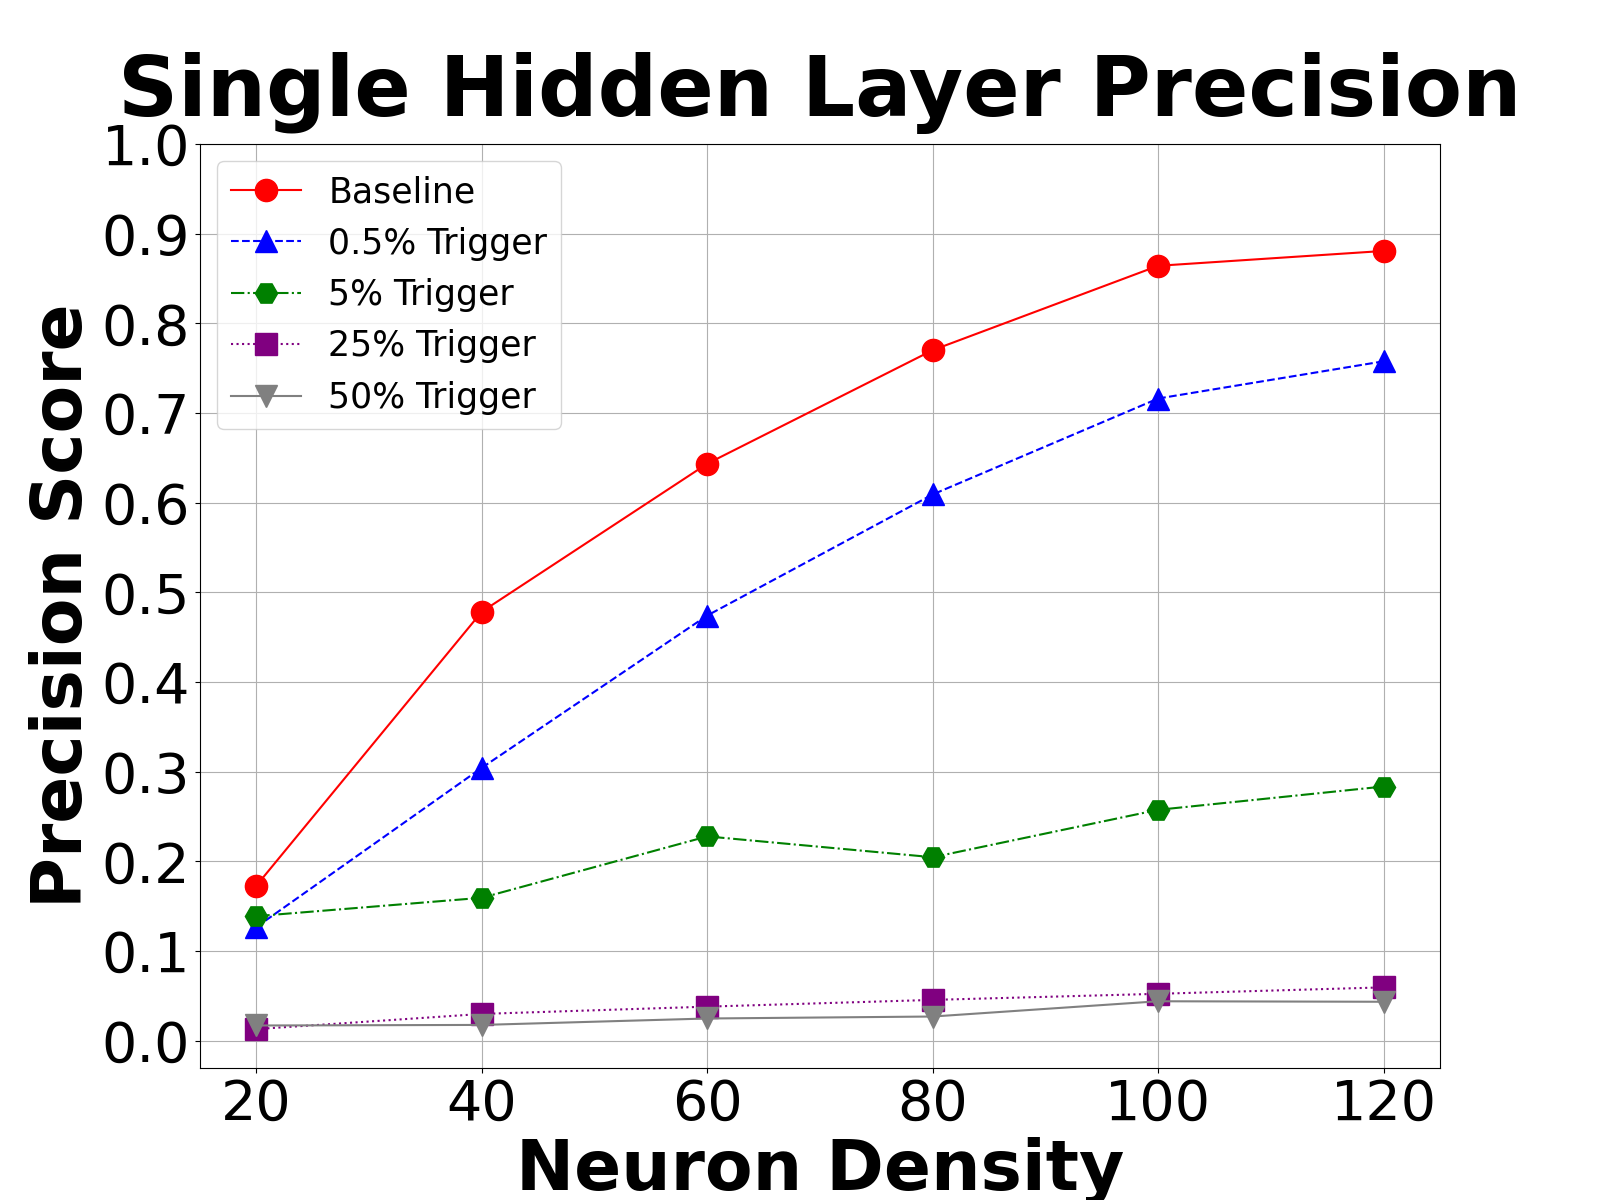
\includegraphics[width=0.45\columnwidth]{Fig/Single_Hidden_Layer_Precision}}
	\subfigure[]{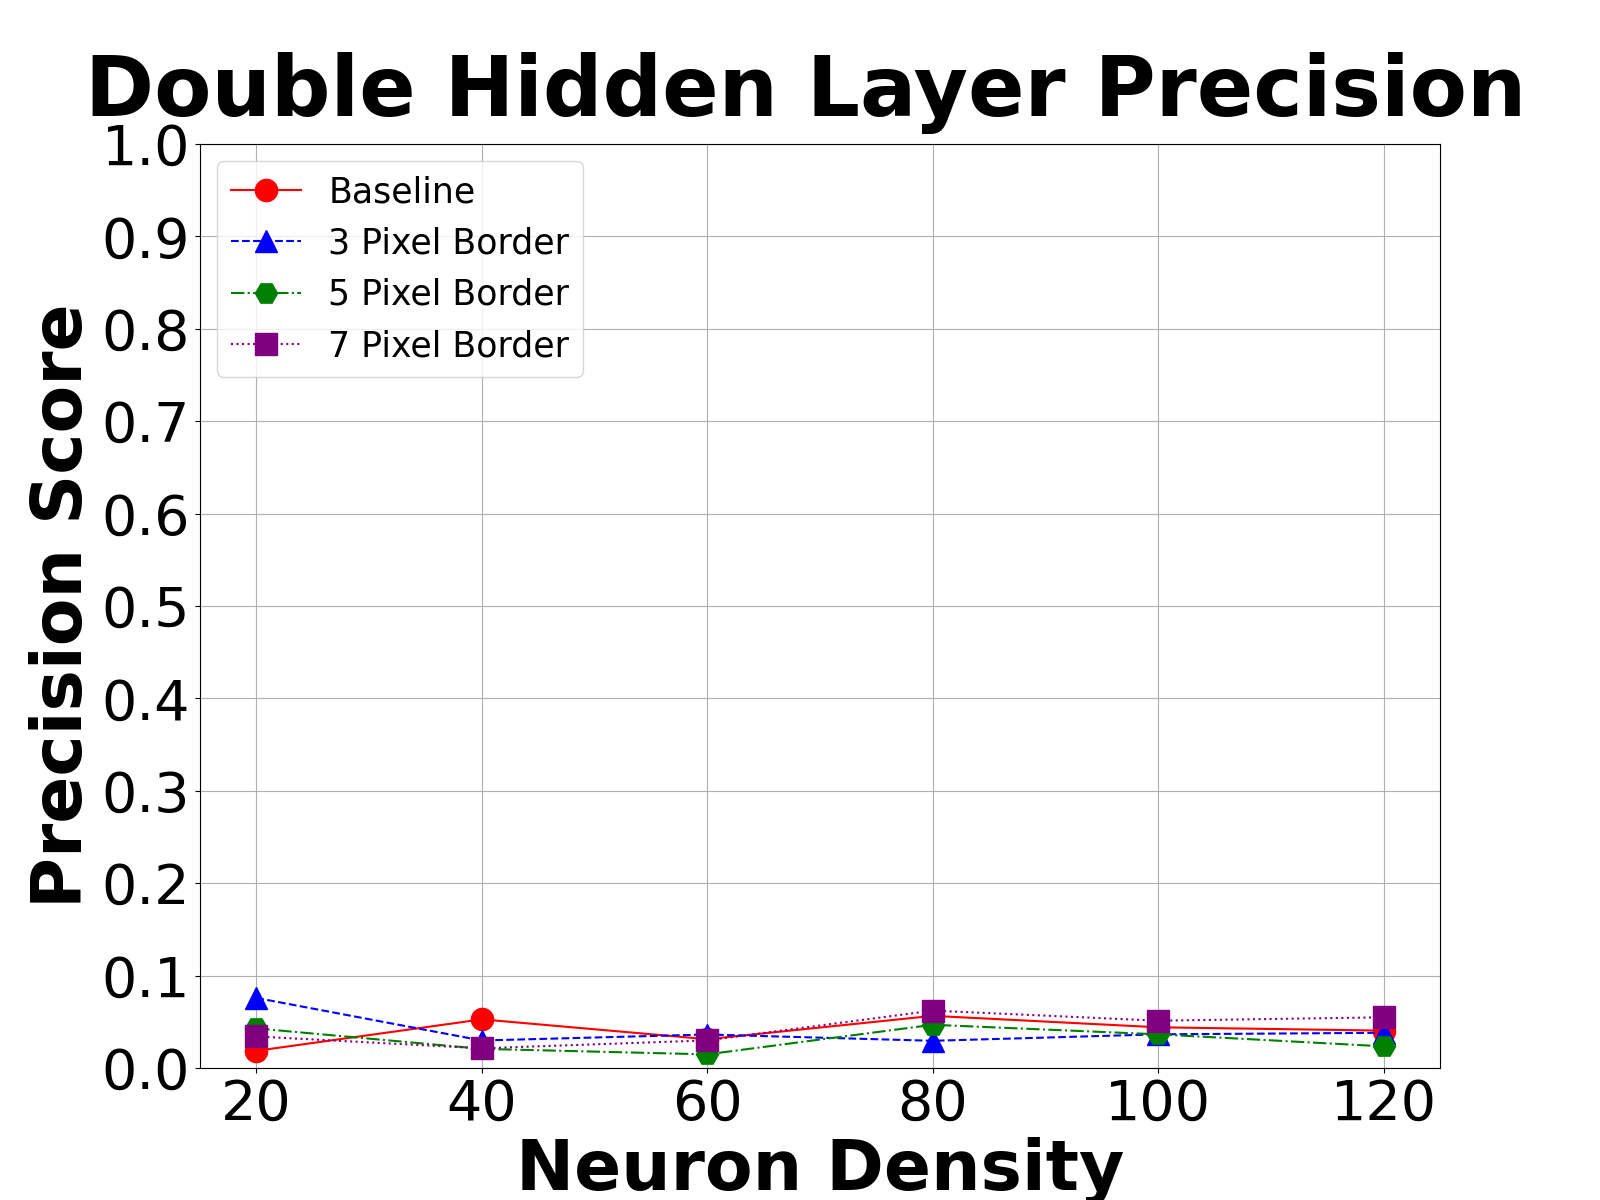
\includegraphics[width=0.45\columnwidth]{Fig/Double_Hidden_Layer_Precision_}}
	\subfigure[]{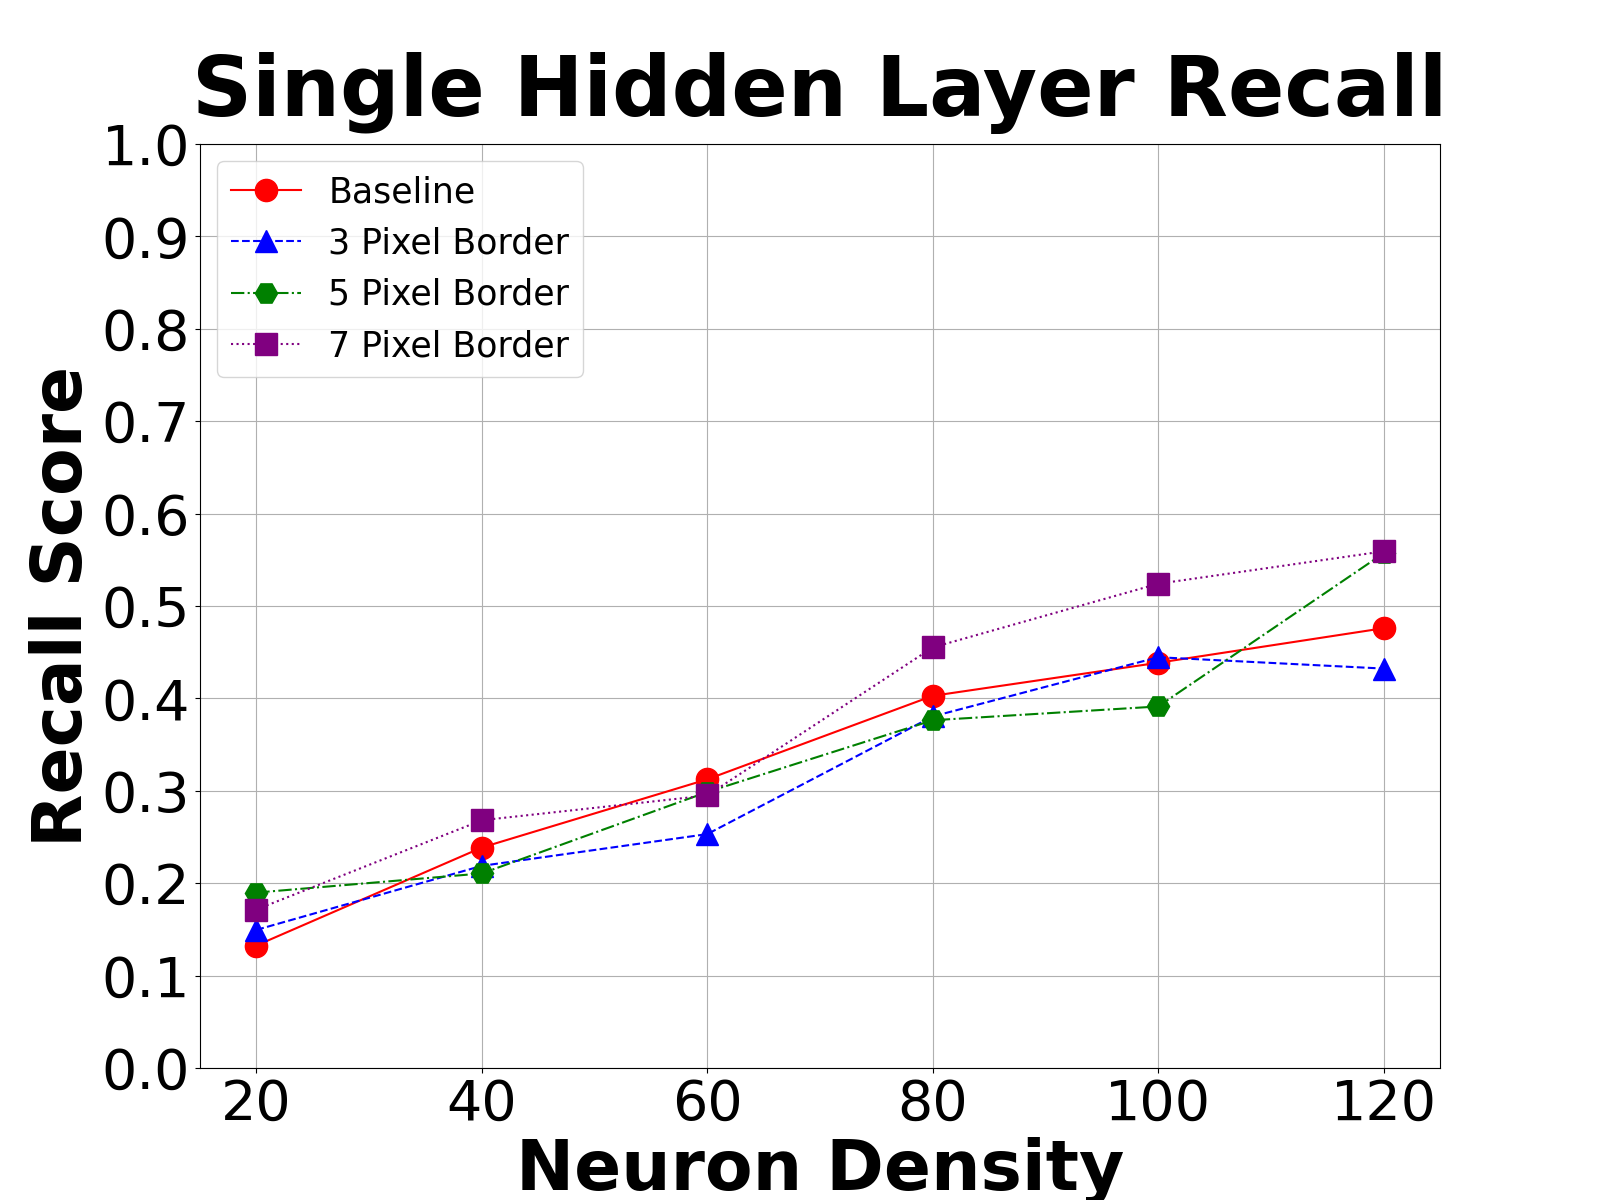
\includegraphics[width=0.45\columnwidth]{Fig/Single_Hidden_Layer_Recall}}
	\subfigure[]{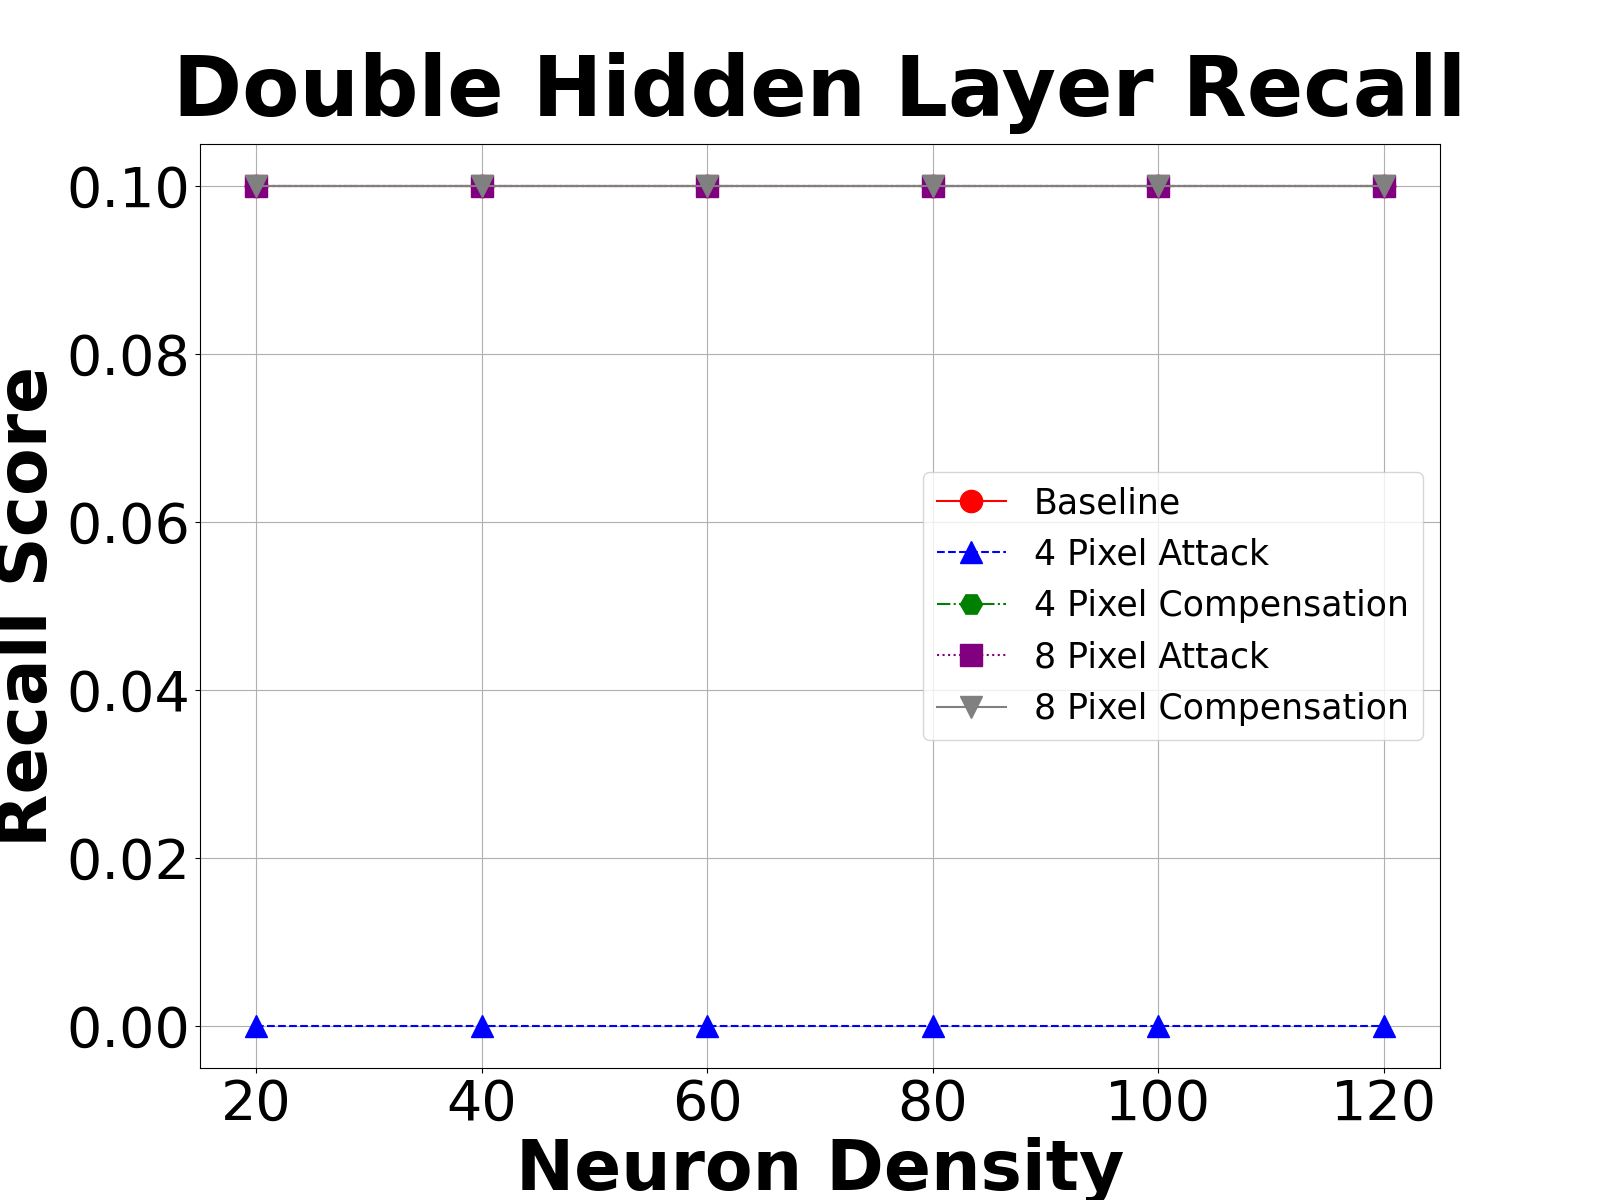
\includegraphics[width=0.45\columnwidth]{Fig/Double_Hidden_Layer_Recall}}
	\caption{Experimental results for baseline, 5\%, 25\% and 50\% attack rates visualized across 6 different neuron densities, and one and two hidden layer models.}
	\label{results}
\end{figure}

\subsubsection{Conclusions from Bit-Muting Attack}

\paragraph*{}The presence of a bit muting attack, with a 5\%,25\% and 50\% trigger condition shows dramatic reductions in the average precisio (c,d) and recall (e,f) scores across all tested classifier models when compared to the un-attacked baseline. Since this type of attack targets the feed-forward mechanism of the network (\ref{feed-forward}), information passed though the network will not produce consistent or reliable outputs, thus prevent the classifier from making appropriate decisions. The exclusion of the most-significant-bit in the double precision floating-point entries in the network destroys the numerical integrity to essentially render this subset of classifier models ineffective entirely, as shown by the inability to minimize the loss function (a,b), as well as poor metric scores. This means if a security measurement were put into place to monitor the behavior of the network, large decreases in the classification scores (precision,recall) and large increases in batch-loss functions, could be used to identify a network which has subject to this type of attack function.

% END LANDON'S ADDITIONS

\end{document}